\documentclass{beamer}
\usetheme{Rochester}
\usepackage{tcolorbox}
\tcbuselibrary{listings}
\usepackage{inconsolata}

\geometry{paperwidth = 4.75in, paperheight = 4.75in}

% Custom U of C color palette
\definecolor{ucMaroon}{RGB}{128,0,0}
\definecolor{ucDarkGray}{RGB}{118,118,118}
\definecolor{ucLightGray}{RGB}{214,214,206}

\setbeamercolor{block title}{fg=white,bg=ucMaroon}
\setbeamercolor{block title alerted}{use=alerted text,fg=white,bg=alerted text.fg}
\setbeamercolor{block title example}{use=example text,fg=white,bg=example text.fg}
\setbeamercolor{block body}{parent=normal text,use=block title,bg=ucLightGray}
\setbeamercolor{block body alerted}{parent=normal text,use=block title alerted,bg=block title alerted.bg}
\setbeamercolor{block body example}{parent=normal text,use=block title example,bg=block title example.bg}

\setbeamercolor{palette primary}{fg=white,bg=ucMaroon}
\setbeamercolor{palette secondary}{fg=white,bg=ucLightGray}
\setbeamercolor{palette tertiary}{fg=white,bg=ucDarkGray}
\setbeamercolor{palette quaternary}{fg=white,bg=black}

\setbeamercolor{sidebar}{bg=ucMaroon}

\setbeamercolor{palette sidebar primary}{fg=ucMaroon}
\setbeamercolor{palette sidebar secondary}{fg=white}
\setbeamercolor{palette sidebar tertiary}{fg=ucMaroon}
\setbeamercolor{palette sidebar quaternary}{fg=white}

\setbeamercolor{titlelike}{parent=palette primary}
\setbeamercolor{itemize item}{fg=ucMaroon}

% Code block formatting. Fragile frames needed for these to work.
\newtcblisting{gitCommand}{
  colframe=black,
  colback=ucLightGray,
  boxrule=1pt,
  arc=2pt,
  left=6pt,
  right=6pt,
  top=6pt,
  bottom=6pt,
  before=\vspace{6pt},
  boxsep=0pt,
  listing only,
  hbox
}


\title{Intermediate Git}
\subtitle{Day 4: Collaborating on GitHub}
\author{Raman A.~Shah}
\date{}

\begin{document}

%% Title
\begin{frame}[plain]
  \titlepage
  \footnotesize{Copyright (c) 2015 by Raman A.~Shah.\\
  \href{https://creativecommons.org/licenses/by-nc-sa/3.0/legalcode}
       {Creative Commons BY-NC-SA 3.0 Unported}.\\
   \href{https://github.com/ramanshah/intermediate\_git}
        {https://github.com/ramanshah/intermediate\_git}}
\end{frame}

%% Back to the Day 2 repo
\begin{frame}[fragile]{Back to the Day 2 repo}
  Do you have a clean sample repository from last time?

  \begin{gitCommand}
cd sample
git status
  \end{gitCommand}

  If not, either clone the course repo or refresh it with
  \texttt{git pull origin master}:

  \begin{gitCommand}
git clone https://github.com/\
ramanshah/intermediate_git.git
  \end{gitCommand}

  Then decompress an updated sample repository:

  \begin{gitCommand}
cp ./intermediate_git/day4/sample.tgz .
tar xzvf sample.tgz
cd sample
git status
  \end{gitCommand}
\end{frame}

%% Manage GitHub: git remote
\begin{frame}[fragile]{Manage GitHub: git remote}
  Try these on your \texttt{intermediate\_git} and \texttt{sample} repos.
  What do you get?

  \begin{gitCommand}
git remote
git remote -v
git remote show origin
  \end{gitCommand}

  To connect your repository to a server:

  \begin{gitCommand}git remote add [remote_name] [url]\end{gitCommand}

  To delete the connection:

  \begin{gitCommand}git remote rm [remote_name]\end{gitCommand}
\end{frame}

%% Remote branches
\begin{frame}[fragile]{Remote branches}
  \begin{gitCommand}[remote]/[branch]\end{gitCommand}

  A read-only pointer to the state of \texttt{[branch]} on \texttt{[remote]}
  the last time you checked.
\end{frame}

%% Tracking branches
\begin{frame}[fragile]{Tracking branches}
  A local branch is sometimes automatically set up to correspond to a remote
  branch:

  \begin{itemize}
    \item When you \texttt{git clone} a repo, \texttt{master} tracks
    \texttt{origin/master}.

    \item When you \texttt{git push} a new branch, that gets set up to track
    as well.
  \end{itemize}

  But to check out someone else's branch from a remote, you have to set up tracking
  yourself:

  \begin{gitCommand}git checkout -b [branch] \
  [remote]/[branch]\end{gitCommand}
\end{frame}

%% Push, fetch, and pull
\begin{frame}[fragile]{Push, fetch, and pull}
  To put local commits on the remote server:

  \begin{gitCommand}git push [remote] [branch]\end{gitCommand}

  To download remote objects:

  \begin{gitCommand}git fetch [remote]\end{gitCommand}

  To download remote objects \emph{and} merge them into your current branch:

  \begin{gitCommand}git pull [remote] [branch]\end{gitCommand}

  \texttt{git pull} = \texttt{git fetch} + \texttt{git merge}!
\end{frame}

%% Everyone's on master
\begin{frame}{Everyone's on master}
  \begin{figure}
    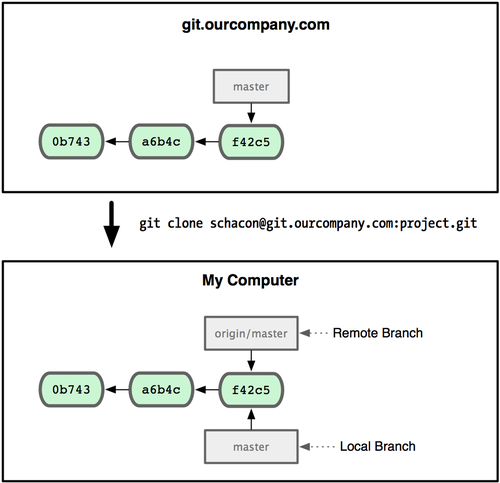
\includegraphics[scale=0.8]{18333fig0322-tn.png}
    \\ A standard \texttt{git clone}.
  \end{figure}
  \footnotesize{Scott Chacon,
    \emph{Pro Git},
    Fig.~3-22.
    \href{https://creativecommons.org/licenses/by-nc-sa/3.0/legalcode}{CC-BY-NC-SA}.
    \href{https://progit.org/}{https://progit.org/}}
\end{frame}

\begin{frame}{Everyone's on master}
  \begin{figure}
    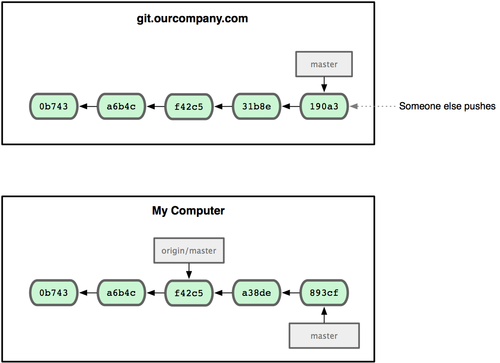
\includegraphics[scale=0.8]{18333fig0323-tn.png}
    \\ Local \texttt{master} has diverged from \texttt{origin/master}.
  \end{figure}
  \footnotesize{Scott Chacon,
    \emph{Pro Git},
    Fig.~3-23.
    \href{https://creativecommons.org/licenses/by-nc-sa/3.0/legalcode}{CC-BY-NC-SA}.
    \href{https://progit.org/}{https://progit.org/}}
\end{frame}

\begin{frame}{Everyone's on master}
  \begin{figure}
    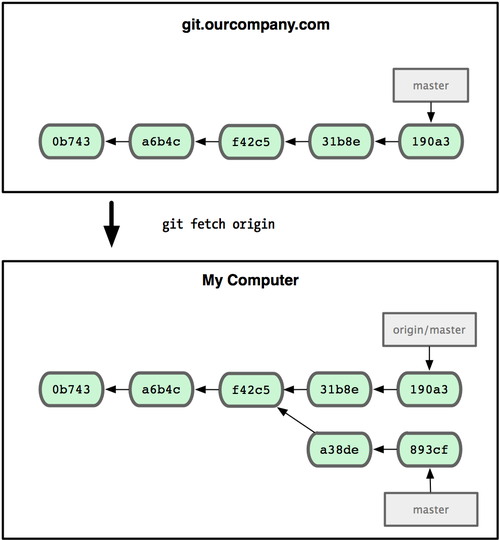
\includegraphics[scale=0.8]{18333fig0324-tn.png}
    \\ You have to \texttt{git fetch}, not \texttt{git pull}.
  \end{figure}
  \footnotesize{Scott Chacon,
    \emph{Pro Git},
    Fig.~3-24.
    \href{https://creativecommons.org/licenses/by-nc-sa/3.0/legalcode}{CC-BY-NC-SA}.
    \href{https://progit.org/}{https://progit.org/}}
\end{frame}

\begin{frame}{Everyone's on master}
  \begin{figure}
    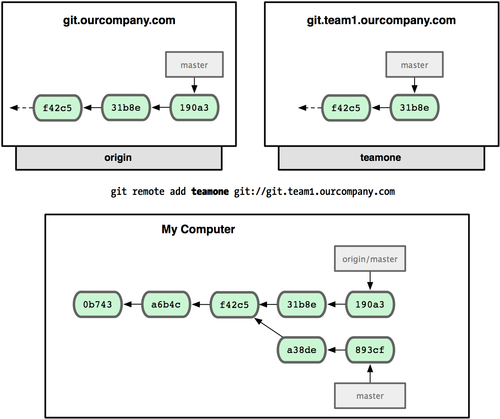
\includegraphics[scale=0.8]{18333fig0325-tn.png}
    \\ You can add a second remote.
  \end{figure}
  \footnotesize{Scott Chacon,
    \emph{Pro Git},
    Fig.~3-25.
    \href{https://creativecommons.org/licenses/by-nc-sa/3.0/legalcode}{CC-BY-NC-SA}.
    \href{https://progit.org/}{https://progit.org/}}
\end{frame}

\begin{frame}{Everyone's on master}
  \begin{figure}
    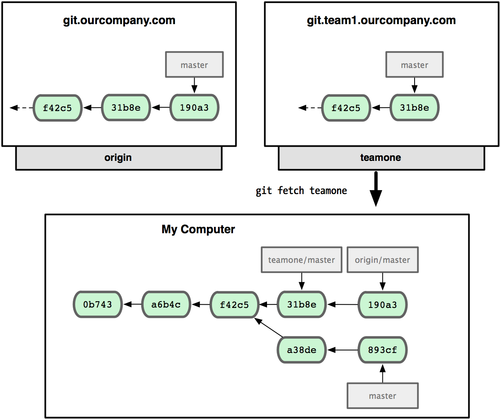
\includegraphics[scale=0.8]{18333fig0326-tn.png}
    \\ Again, \texttt{git fetch}, not \texttt{git pull}, is appropriate.
  \end{figure}
  \footnotesize{Scott Chacon,
    \emph{Pro Git},
    Fig.~3-26.
    \href{https://creativecommons.org/licenses/by-nc-sa/3.0/legalcode}{CC-BY-NC-SA}.
    \href{https://progit.org/}{https://progit.org/}}
\end{frame}

%% Recommendation
\begin{frame}{Recommendation}
  \huge {
  When collaborating, don't work on \texttt{master}.
  \\
  If you do, avoid \texttt{git pull}.
}
\end{frame}

%% Pull requests - can push
\begin{frame}{Pull requests---can push}
  Why wouldn't you just push to \texttt{master}?

  \begin{itemize}
    \item Pull requests give a mechanism for peer review of code.
    \item Others might expect \texttt{master} to be working or stable.
    \item The \texttt{master} branch might need to be ready to
          go, \emph{e.g.}, deployable.
  \end{itemize}

  Even if you have push access, submit changes as pull requests as a
  matter of \emph{safety} and \emph{etiquette}.
\end{frame}

%% Pull requests with push access flipbook
\begin{frame}{Pull requests---can push}
  \begin{figure}
    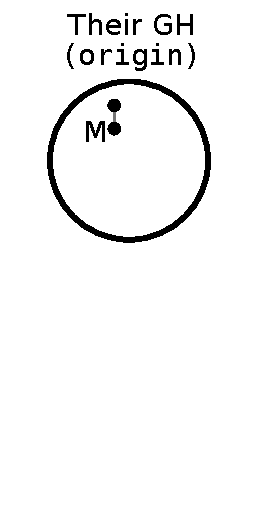
\includegraphics{push_001.pdf}
    \\ Someone has a project.
    \\ They give you push access.
  \end{figure}
\end{frame}

\begin{frame}{Pull requests---can push}
  \begin{figure}
    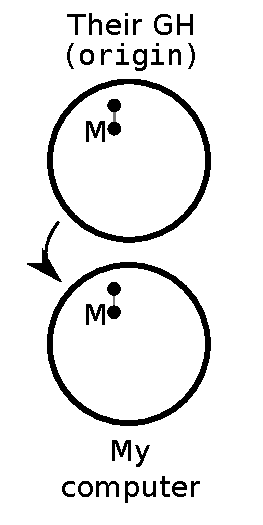
\includegraphics{push_002.pdf}
    \\ \texttt{git clone [url]}
    \\ \texttt{}
  \end{figure}
\end{frame}

\begin{frame}{Pull requests---can push}
  \begin{figure}
    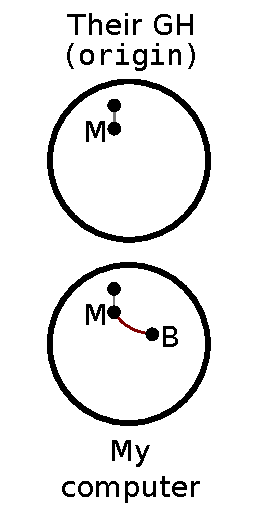
\includegraphics{push_003.pdf}
    \\ \texttt{git checkout -b my\_branch}
    \\ Do work; make commits.
  \end{figure}
\end{frame}

\begin{frame}{Pull requests---can push}
  \begin{figure}
    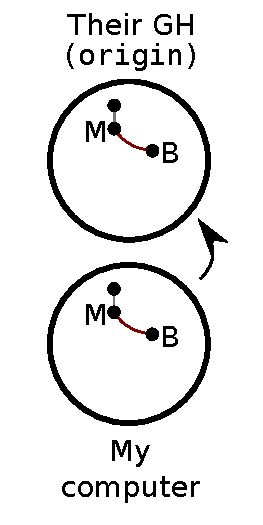
\includegraphics{push_004.pdf}
    \\ \texttt{git push origin my\_branch}
    \\ \texttt{}
  \end{figure}
\end{frame}

\begin{frame}{Pull requests---can push}
  \begin{figure}
    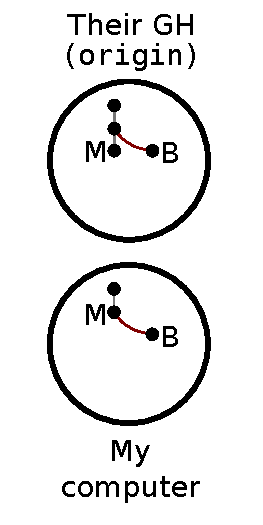
\includegraphics{push_005.pdf}
    \\ They put some new work on \texttt{master}.
    \\ \texttt{}
  \end{figure}
\end{frame}

\begin{frame}{Pull requests---can push}
  \begin{figure}
    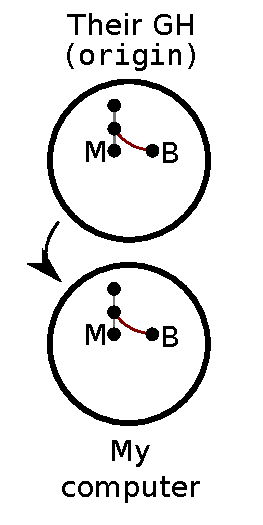
\includegraphics{push_006.pdf}
    \\ \texttt{git checkout master}
    \\ \texttt{git pull origin master}
  \end{figure}
\end{frame}

\begin{frame}{Pull requests---can push}
  \begin{figure}
    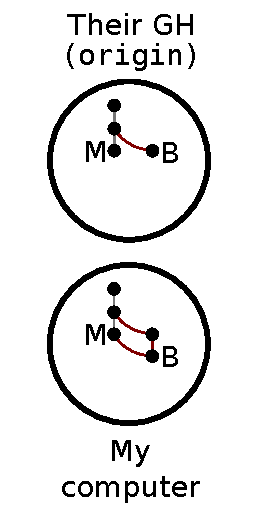
\includegraphics{push_007.pdf}
    \\ \texttt{git checkout my\_branch}
    \\ \texttt{git merge master}
  \end{figure}
\end{frame}

\begin{frame}{Pull requests---can push}
  \begin{figure}
    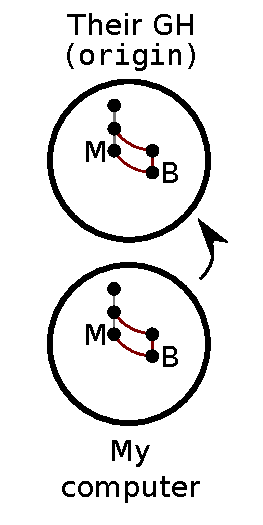
\includegraphics{push_008.pdf}
    \\ \texttt{git push origin my\_branch}
    \\ \texttt{}
  \end{figure}
\end{frame}

\begin{frame}{Pull requests---can push}
  \begin{figure}
    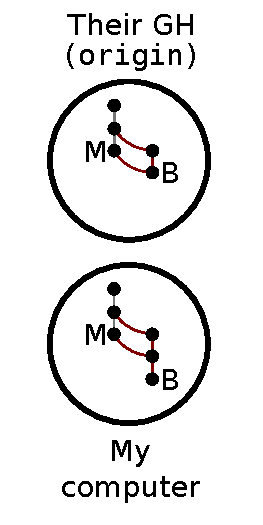
\includegraphics{push_009.pdf}
    \\ Click ``New Pull Request''
    \\ Get comments; do work; make commits.
  \end{figure}
\end{frame}

\begin{frame}{Pull requests---can push}
  \begin{figure}
    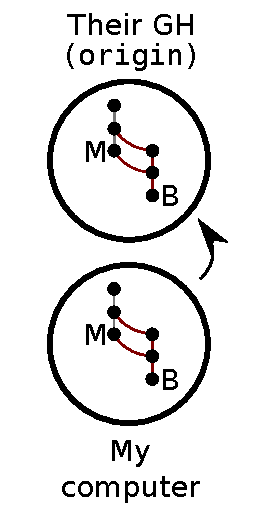
\includegraphics{push_010.pdf}
    \\ \texttt{git push origin my\_branch}
    \\ \texttt{}
  \end{figure}
\end{frame}

\begin{frame}{Pull requests---can push}
  \begin{figure}
    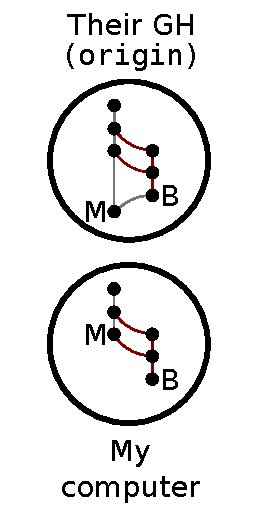
\includegraphics{push_011.pdf}
    \\ ``LGTM''---``Looks Good To Me.''
    \\ You click ``Merge Pull Request.''
  \end{figure}
\end{frame}

\begin{frame}{Pull requests---can push}
  \begin{figure}
    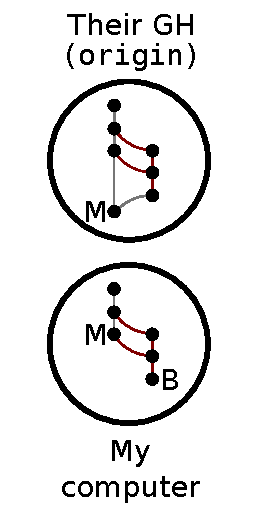
\includegraphics{push_012.pdf}
    \\ You click ``Delete Branch.''
    \\ \texttt{}
  \end{figure}
\end{frame}

\begin{frame}{Pull requests---can push}
  \begin{figure}
    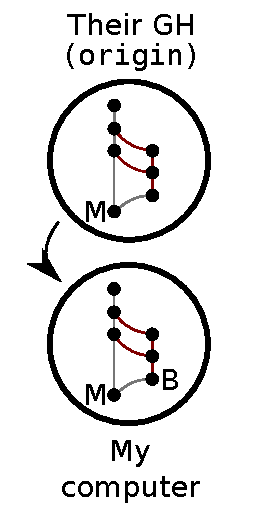
\includegraphics{push_013.pdf}
    \\ \texttt{git checkout master}
    \\ \texttt{git pull origin master}
  \end{figure}
\end{frame}

\begin{frame}{Pull requests---can push}
  \begin{figure}
    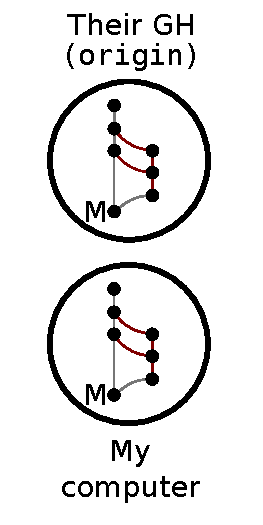
\includegraphics{push_014.pdf}
    \\ \texttt{git branch -d my\_branch}
    \\ Done!
  \end{figure}
\end{frame}

%% Pull requests - can't push
\begin{frame}{Pull requests---can't push}
  If you don't have push access, you have to:

  \begin{itemize}
    \item \emph{Fork} the repo on GitHub.
    \item Curate your fork so that the changes in the fork can be
          applied to the original repo in a single pull without
          merge conflicts.
    \item In some projects, rebase your work so that the commits are
          ``nice'' and result in a fast-forward merge.
  \end{itemize}

  This is the default case in open source work.
\end{frame}

%% Pull requests without push access flipbook
\begin{frame}{Pull requests---can't push}
  \begin{figure}
    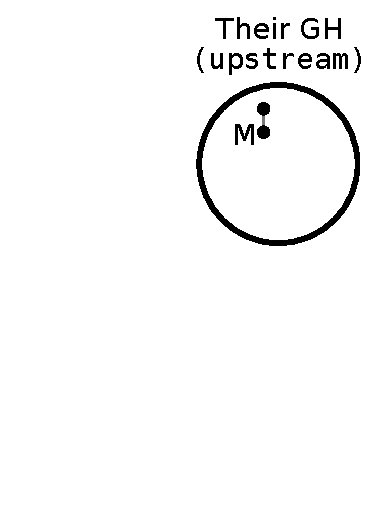
\includegraphics{fork_001.pdf}
    \\ Someone has a project.
    \\ \texttt{}
  \end{figure}
\end{frame}

\begin{frame}{Pull requests---can't push}
  \begin{figure}
    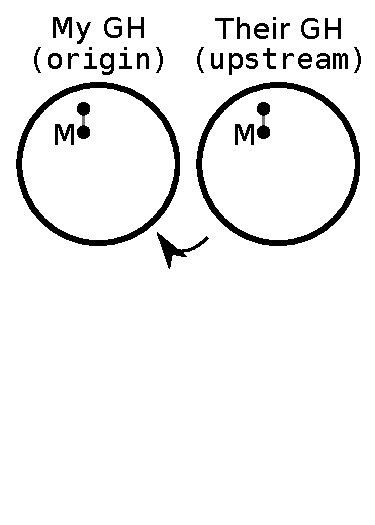
\includegraphics{fork_002.pdf}
    \\ Click ``Fork'' on GitHub.
    \\ \texttt{}
  \end{figure}
\end{frame}

\begin{frame}{Pull requests---can't push}
  \begin{figure}
    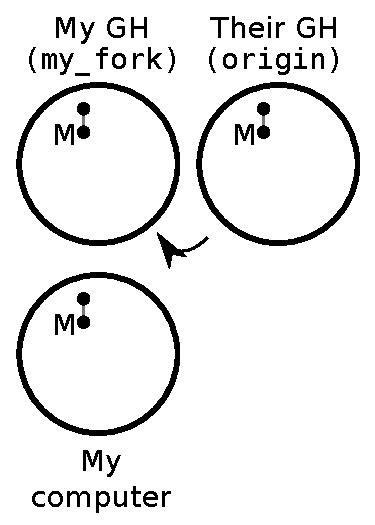
\includegraphics{fork_003.pdf}
    \\ \texttt{git clone [my\_url]}
    \\ \texttt{git remote add upstream [their\_url]}
  \end{figure}
\end{frame}

\begin{frame}{Pull requests---can't push}
  \begin{figure}
    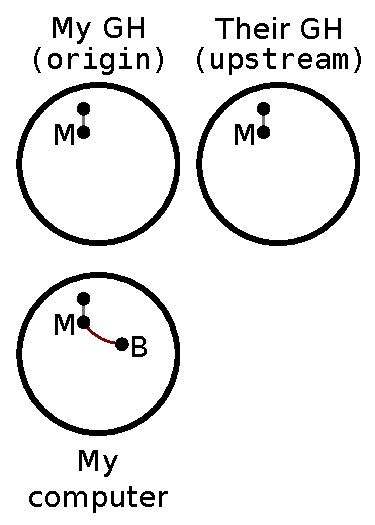
\includegraphics{fork_004.pdf}
    \\ \texttt{git checkout -b my\_branch}
    \\ Do work; make commits.
  \end{figure}
\end{frame}

\begin{frame}{Pull requests---can't push}
  \begin{figure}
    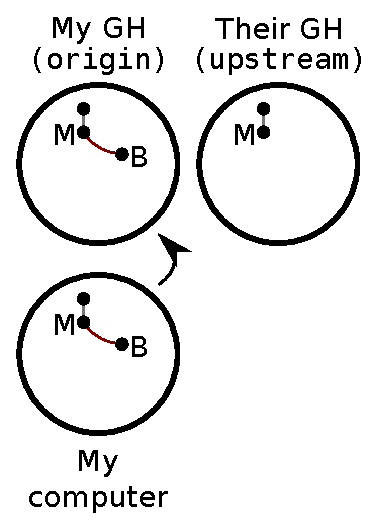
\includegraphics{fork_005.pdf}
    \\ \texttt{git push origin my\_branch}
    \\ \texttt{}
  \end{figure}
\end{frame}

\begin{frame}{Pull requests---can't push}
  \begin{figure}
    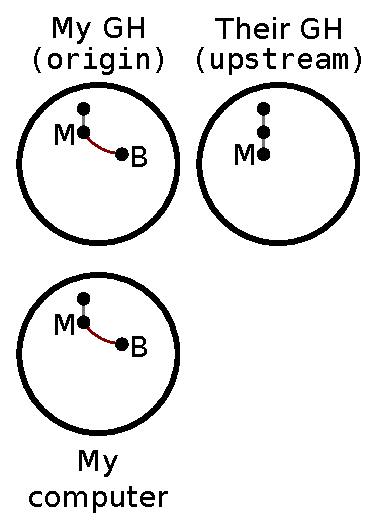
\includegraphics{fork_006.pdf}
    \\ They put some new work on \texttt{master}.
    \\ \texttt{}
  \end{figure}
\end{frame}

\begin{frame}{Pull requests---can't push}
  \begin{figure}
    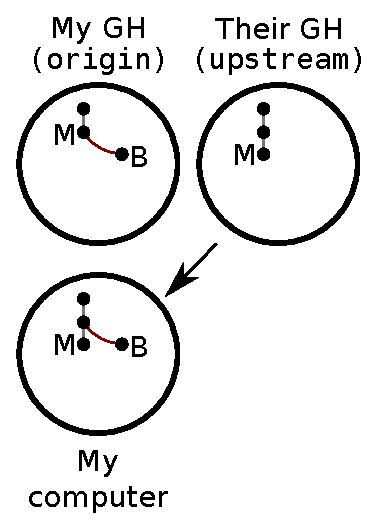
\includegraphics{fork_007.pdf}
    \\ \texttt{git checkout master}
    \\ \texttt{git pull upstream master}
  \end{figure}
\end{frame}

\begin{frame}{Pull requests---can't push}
  \begin{figure}
    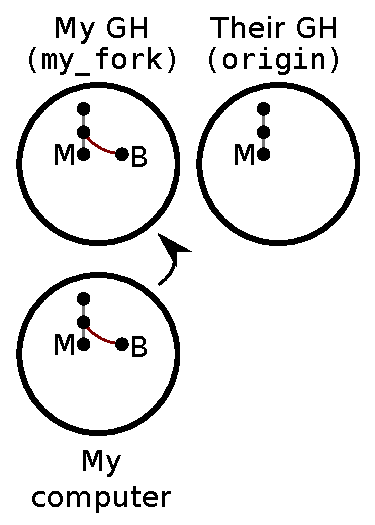
\includegraphics{fork_008.pdf}
    \\ \texttt{git push origin master}
    \\ \texttt{}
  \end{figure}
\end{frame}

\begin{frame}{Pull requests---can't push}
  \begin{figure}
    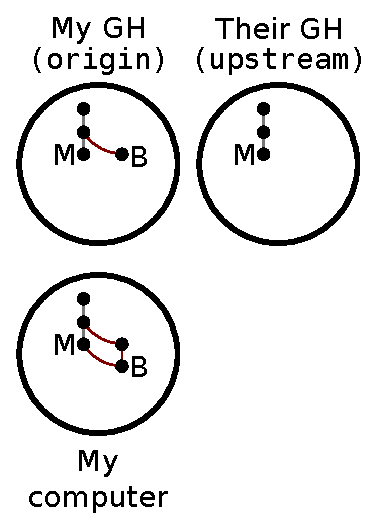
\includegraphics{fork_009.pdf}
    \\ \texttt{git checkout my\_branch}
    \\ \texttt{git merge master}
  \end{figure}
\end{frame}

\begin{frame}{Pull requests---can't push}
  \begin{figure}
    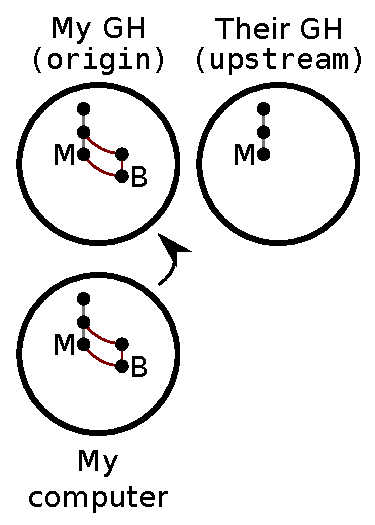
\includegraphics{fork_010.pdf}
    \\ \texttt{git push origin my\_branch}
    \\ \texttt{}
  \end{figure}
\end{frame}

\begin{frame}{Pull requests---can't push}
  \begin{figure}
    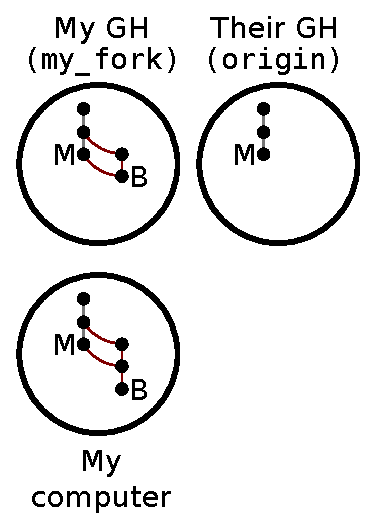
\includegraphics{fork_011.pdf}
    \\ Click ``New Pull Request''
    \\ Get comments; do work; make commits.
  \end{figure}
\end{frame}

\begin{frame}{Pull requests---can't push}
  \begin{figure}
    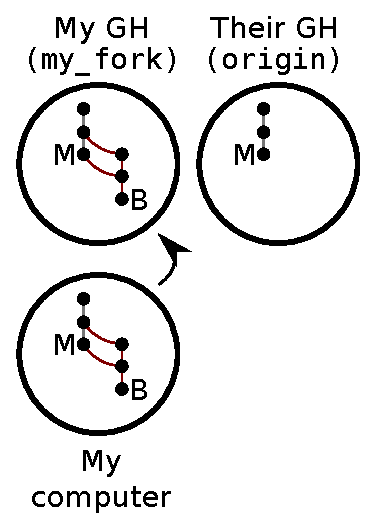
\includegraphics{fork_012.pdf}
    \\ \texttt{git push origin my\_branch}
    \\ \texttt{}
  \end{figure}
\end{frame}

\begin{frame}{Pull requests---can't push}
  \begin{figure}
    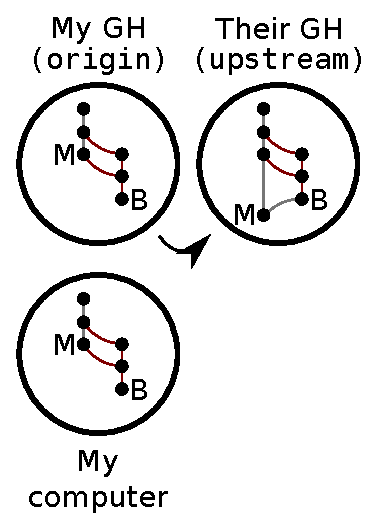
\includegraphics{fork_013.pdf}
    \\ They're happy. They click ``Merge Pull Request.''
  \end{figure}
\end{frame}

\begin{frame}{Pull requests---can't push}
  \begin{figure}
    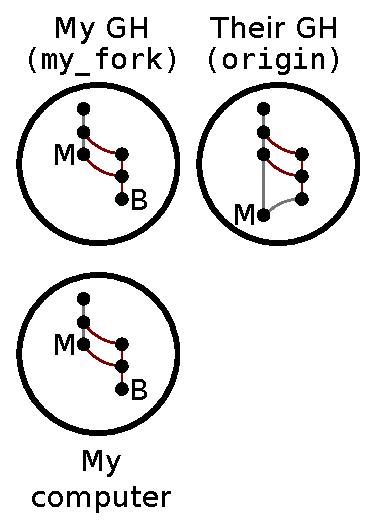
\includegraphics{fork_014.pdf}
    \\ They click ``Delete Branch.''
    \\ \texttt{}
  \end{figure}
\end{frame}

\begin{frame}{Pull requests---can't push}
  \begin{figure}
    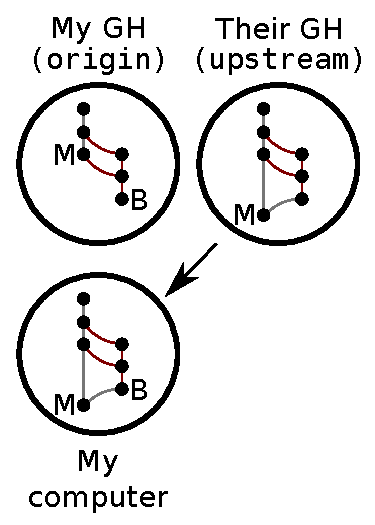
\includegraphics{fork_015.pdf}
    \\ \texttt{git checkout master}
    \\ \texttt{git pull upstream master}
  \end{figure}
\end{frame}

\begin{frame}{Pull requests---can't push}
  \begin{figure}
    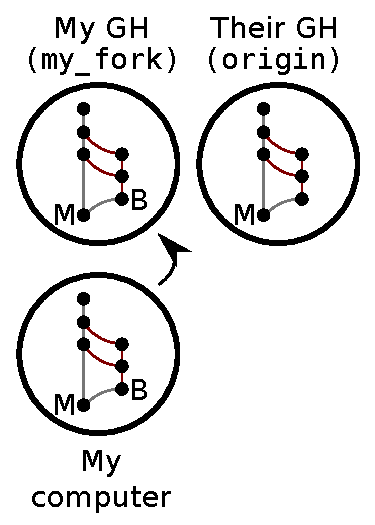
\includegraphics{fork_016.pdf}
    \\ \texttt{git push origin master}
    \\ \texttt{}
  \end{figure}
\end{frame}

\begin{frame}{Pull requests---can't push}
  \begin{figure}
    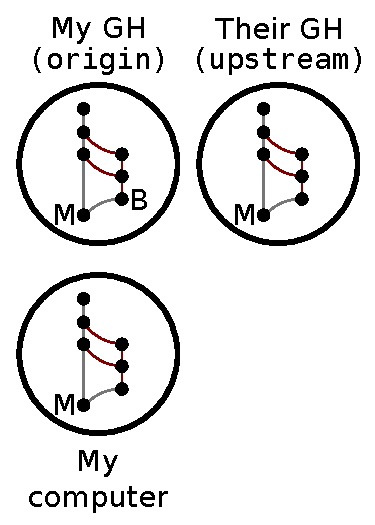
\includegraphics{fork_017.pdf}
    \\ \texttt{git branch -d my\_branch}
    \\ \texttt{}
  \end{figure}
\end{frame}

\begin{frame}{Pull requests---can't push}
  \begin{figure}
    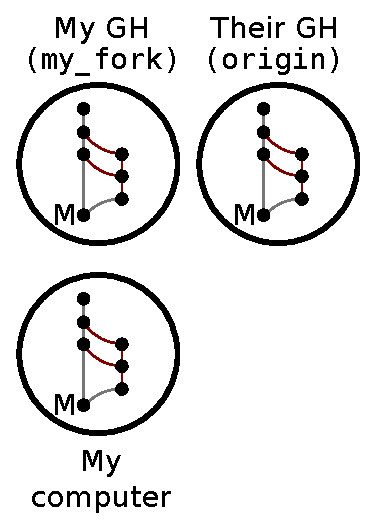
\includegraphics{fork_018.pdf}
    \\ \texttt{git push origin :my\_branch}
    \\ Done!
  \end{figure}
\end{frame}

%% Keep pull requests small!
\begin{frame}{Keep pull requests small!}
  Shorter pull requests involve:

  \begin{itemize}
    \item Less \emph{time} to diverge from \texttt{master}---hence
          fewer merge conflicts
    \item Less \emph{cognitive load} for the developer and maintainer
          to comprehend and communicate the reasoning behind the
          changes
  \end{itemize}

  My personal rule of thumb is that a pull request is too big if you exceed:

  \begin{itemize}
    \item Roughly one week of active development time
    \item Roughly 150 lines of source code
  \end{itemize}
\end{frame}

%% Conclusion
\begin{frame}{Conclusion}
  \begin{figure}
    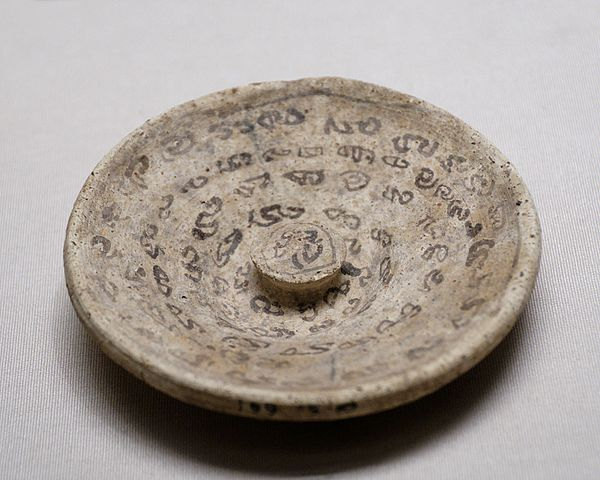
\includegraphics[scale=0.82]{magic_lid.jpg}
  \end{figure}
\end{frame}

\end{document}
